%!TEX root = ../thesis.tex

\chapter{引言}

\section{我国信用债违约历史}

自 2014 年“11 超日债”违约以来,我国信用债市场中投资者“刚性兑付”的“信仰”逐步动摇、破灭。及至 2021 年,永城煤电、华晨宝马的违约打破了人们对 AAA 级国企的“刚兑信仰”,恒大、海航违约使人们意识到并不存在所谓“大而不倒”,投资者对债券投资逐步恢复理性,我国债券市场也愈发成熟,对债券违约的认识也愈发深刻。近年来一些典型的债券违约事件如表\ref{tab:defaults_in_history}所示。

违约是经济中的正常现象。过去,我国信用债市场维持着“刚兑”神话,并非正常现象,而是风险无序累积的过程。在经济周期的起伏过程中,企业经营失败是正常的现象。通过违约释放掉部分信用风险,恰恰能降低大规模系统性金融风险发生的概率。违约可以使泡沫膨胀到更大前的提前破裂。如近期的房地产企业的加速出清,是过去房企高杠杆经营扩张的反噬。如果长时间维持高杠杆经营,居民部门负债率高企,地产商开发贷终将难以维续,势必会对银行系统造成很大的威胁,进而影响我国金融稳定。
\begin{table}[h]
	\caption{近年来部分著名的违约}
	\centering
	\begin{tabular}{lccc}
		债券             & 违约日期   & 原因               & 影响                   \\ \hline
		11 超日债        & 2014-03-05 & 过度扩张资金链断裂 & 打破刚兑的开始         \\
		11天威MTN2       & 2015-04-21 & 经营亏损资不抵债   & 打破国企刚兑           \\
		14波鸿CP001      & 2015-04-12 & “技术性”违约       & 首例“技术性违约”       \\
		15五洋债         & 2018-08-16 & 欺诈发行           & 首例公司债券欺诈发行案 \\
		16民生投资PPN001 & 2019-01-29 & “技术性”违约       & AAA 债券违约第一例     \\
		20永煤SCP003     & 2020-11-26 & 逃废债             & 河南全省融资环境恶化   \\
		15天安人寿       & 2020-12-29 & 股东抽血           & 金融机构破刚兑付       \\
		17幸福基业MTN001 & 2021-02-27 & 过度扩张遇宏观调控 & 地产债违约潮的开始     \\
	\end{tabular}
	\label{tab:defaults_in_history}
\end{table}

套用托尔斯泰的开场白,成功的企业都是相似的,失败的企业却各有各的不同,这句话似乎适用于债券市场。
我国债券市场的交易额相较于债券市场的体量非常小,违约是小概率事件,成功兑付的债券似乎是天经地义,走向违约的企业各有各的说辞:或称技术原因场外兑付(中融新大),或怨评级公司下调评级(花样年、新力),或称公司流动性遇到了暂时的困难(恒大)。债务违约的危害是多层次的:对投资人意味着不小的损失;对发行人意味着丧失外部融资功能、经营难以维系;此外违约还有一定的外部性:如果处理不好如永煤逃废债可能会影响区域乃至全国的投融资环境,进而会对整个经济体造成影响。

以史为鉴,可知兴替。当前时点债券市场格外引人注目,深陷其中的不少房企是上下游工人衣食所系、购房者家屋所托。如何化解违约带来的风险考验我国金融市场的能力。
本文计划研究企业在债券市场上为何走向违约,从债券违约影响因素出发,研究我国债券市场违约债券的共性特征,并通过机器学习的方式佐证、拓展计量模型,以期对债券市场有一个比较好的刻画。

\section{文献综述}
\label{sec:zs}
对于企业违约,不少学者提出过非常深刻的见解。

信用评级是企业违约风险最直观的表述之一,不少学者从信用评级的角度研究企业违约。难以否认的是,我国信用评级市场存在很大的不完善,信用评级比较扭曲,如图\ref{fig:rating}所示,新发行债券有一半为最高评级 AAA 。
\begin{figure}[h]
	\centering
	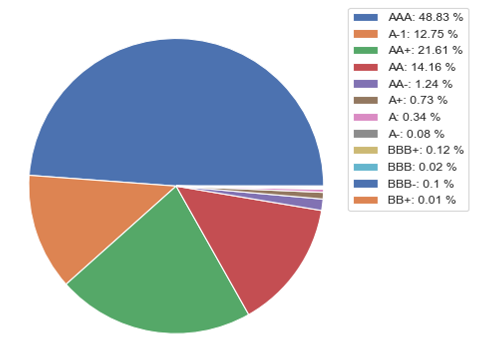
\includegraphics[width=0.9\linewidth]{./data/rating_from_2014.png}
	\caption{\label{fig:rating}信用债发行评级统计}
\end{figure}
这很大程度上是由于发行人付费的模式引起的。\Textcite{吴育辉2020} 指出,“发行人付费”模式下,信用评级虽然可以在一定程度上包含公司的内部私有信息,但由于独立性缺失问题,其总体的信用评级质量仍然低于“投资人付费”模式下的信用 评级质量。此外评级机构竞争为了获得收入也会对公司虚高评级,这是国际著名的评级机构也无法避免的\Parencite{opp2013rating}。
有些评级为了维护发行人利益,初始给予很高的评级,随后在违约事件已经板上钉钉时几天内连续下调原先的虚高评级至垃圾级,如图 \ref{fig:rating_of_zg}  所示。\Textcite{陈关亭2021多重信用评级与债券融资成本}就对这种现象发出强烈抨击,认为竞争付费导致评级机构存在评级偏差,部分评级机构声誉较差。这种情况即便在违约发生后,涉事评级机构非但不考虑模型是否有偏误,反而为了争取市场份额而放宽标准、提高评级\cite{黄小琳2017债券违约对涉事信用评级机构的影响}。
事实上,被\Textcite{王雄元2013声誉机制}列为低声誉评级机构的大公国际,因涉嫌帮助欺诈发行“五洋债”,应承担 10\% 的连带责任赔偿 7400 万元。但大公竟称“公司已经发不出工资,顶多赔偿150万元”,最终被列入失信被执行人,可见某些评级机构对自身声誉的重视程度。
\begin{figure}[h]
	\centering
	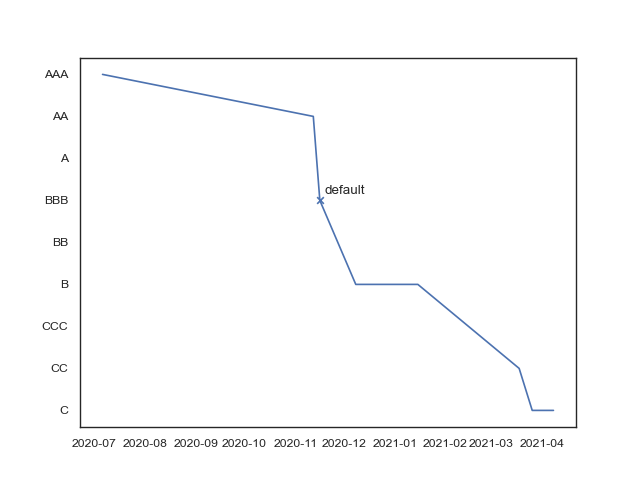
\includegraphics[width=0.9\linewidth]{./data/rating_of_zg.png}
	\caption{某评级公司对某违约发行人的历史评级}
	\label{fig:rating_of_zg}
\end{figure}
不仅仅是国内,国外也有学者提出评级可能是最差的信用评估方式\cite{blochlinger2018ratings},债券交易的价格可能更有效\cite{badoer2019relevance}。我国也是如此,债券价格大幅偏离估值往往是违约的先兆,一般认为面值100的债券价格下跌至60元左右相当于即将违约,已经违约的债券往往价格只有20元左右。但单纯以价格异动预测违约存在不少假阳性情况,特别是在城投债中,弱省市的城投债成交收益率有时能达到20\%乃至更高。

公司层面的研究很多还有涉及到公司治理方面的研究。
\Textcite{林晚发2018高管任职经历的得与失}从高管任职经历出发,发现有高管担任过人大代表或政协委员的企业债券发行成功率更高,
\Textcite{anginer2018corporate}提出一个涵盖管理、约束、独立三方面指标的公司治理指标,并指出公司治理增加一个标准差使银行的违约距离指标降低了 0.14 个标准差。
\Textcite{ding2021corporate}和\Textcite{subrahmanyam2017credit}分别从疫情和引入 CDS 对公司治理的影响出发,研究外生冲击由于公司治理能力的差异影响偿债能力的差异。

宏观层面
\Textcite{bai2019common}和\Textcite{bali2021macroeconomic}分别从宏观经济下行和宏观经济不确定性出发,研究宏观环境对于公司债利差的影响。宏观政策角度,
\Textcite{梅冬州2021财政扩张}和\Textcite{2020Fiscal} 则认为财政扩张导致挤出效应,从而民企面临融资困境,进而违约率上升,利差走阔。
\Textcite{王博2019货币政策不确定性}指出货币政策不确定性的增加会带来违约风险的上升。此外,流动性可能会影响违约\cite{brogaard2017stock},更高的流动性可以通过提高价格效率来降低违约风险,或者通过放松投资者的退出能力来改善公司治理。

最后还有风险传染角度,有关研究主要集中在系统性风险传染。
\Textcite{苟文均2016债务杠杆与系统性风险传染机制}基于 CCA 模型,提出杠杆率应从较高居民转移至政府等低杠杆部门,以降低违约风险。
\Textcite{2020Do} VAR 模型,认为几乎所有的系统性风险指标对对违约率都有预测能力。
\Textcite{azizpour2018exploring}则认为公司之间的财务、法律或业务关系可能充当风险分散的渠道,通过捕捉系统性风险和这种非系统性的聚类,可以几乎完美地匹配了的时间变化结果所隐含的时间变化的违约计数和违约时间的理论分布。
